\clearpage
\maketitlesupplementary

% ============================================================
% A. Exact prompts and decoding
% ============================================================
\section{Exact Prompts, Decoding, and Parsing}
\label{app:prompts}

\textbf{VSR plain prompt} (identical for 2B and 7B, all conditions;
`\{statement\}' is the VSR caption):
\begin{verbatim}
Look at the image carefully.

Statement: "{statement}"

Is this statement true or false?

Answer with exactly one word:
True or False.
\end{verbatim}

\textbf{2B structured-decomposition prompt} (2B only; single run):
\begin{verbatim}
Look carefully at the image.

Statement:
"{statement}"

Determine whether the statement is true
by doing the following:
1. Identify the subject object.
2. Identify the reference object.
3. Determine the position and
   orientation of the subject relative
   to the reference object.
4. Pay careful attention to left/right,
   front/back, viewpoint, and
   orientation.
5. Decide whether the stated spatial
   relationship matches the image.

Answer with exactly one word:
True or False.
\end{verbatim}

\textbf{SITE multiple-choice prompt} (replicated from the official
lmms-eval task \texttt{sitebench/utils.py}):
\begin{verbatim}
# image examples (one <image> token per visual):
<image>...
Question: {question}
Options:
A: {opt0}
B: {opt1}
...
Give me the answer letter directly.
The best answer is:

# video examples (pre-prompt):
Select the best answer to the following
multiple-choice question based on the
video. Respond with only the letter
of the correct option.
Question: {question}
Options:
A: ...
B: ...
...
Give me the answer letter directly.
The best answer is:
\end{verbatim}

\textbf{Decoding.} All generations are greedy: $\mathrm{do\_sample}{=}$False,
temperature 0, top-$p$ 1.0. $\mathrm{max\_new\_tokens}$: 5 for the 2B wrapper,
128 for 7B VSR runs, 16 for SITE (change validated parse-identical on 125/125
held-out outputs before adoption; recorded in the SITE run metadata).

\textbf{Parsing.} VSR outputs are parsed with an anchored case-insensitive
regex (\texttt{src/evaluation/parser.py}): strips prefixes
(`the answer is', `answer:', `response:', `output:') and trailing
punctuation; accepts exact `true/yes/correct' or `false/no/incorrect' forms;
substring fallback only when exactly one of `true'/'false' appears. Invalid
outputs are counted as wrong, never guessed; invalid rate is 0 on all reported
runs. SITE outputs use the official \texttt{parse\_multi\_choice\_response}
(letter); unparseable responses are counted incorrect and reported.

% ============================================================
% B. Training configurations
% ============================================================
\section{Training and Adapter Configurations}
\label{app:training}

All LoRA conditions share: $r{=}8$, $\alpha{=}16$, dropout 0.05, AdamW
lr $10^{-4}$, weight decay 0.01, linear warmup 10\% of steps, 2 epochs,
bf16, gradient checkpointing, gradient clipping 1.0, vision tower frozen.
Adapter configs are committed at \texttt{checkpoints/*/final/adapter\_config.json}.

\begin{table*}[h]
\centering
\footnotesize
\setlength{\tabcolsep}{4pt}
\begin{tabular}{llccc}
\toprule
Condition & LoRA targets & Trainable & Batch & Manifest \\
\midrule
2B General & LM q/k/v/o & $\sim$2.3M & microbatch 4$\times$4 & general (2{,}000) \\
2B Targeted & LM q/k/v/o & $\sim$2.3M & same & targeted (2{,}000) \\
7B LM-only & LM q/k/v/o & $\sim$0.3M & 1 & general (2{,}000) \\
7B HardNeg & LM q/k/v/o & $\sim$0.3M & 1 & hard-negative (2{,}000) \\
7B Projector & \texttt{visual.merger.mlp.0/2} & 152K & 1 & general (2{,}000) \\
7B Vision+Proj & merger + blocks 24--31 & 1.46M & 1 & general (2{,}000) \\
\bottomrule
\end{tabular}
\caption{LoRA conditions and their target modules.}
\label{tab:adapters}
\end{table*}

\textbf{Manifest construction.} \emph{General}: 2{,}000 statements sampled from
the VSR train split. \emph{Targeted}: orientation-over-sampled subset of the
same split. \emph{Hard-negative}: the orientation block of the general manifest
is replaced by audited-clean originals plus paired hard negatives
(facing$\leftrightarrow$facing away from; parallel$\leftrightarrow$perpendicular)
with flipped labels; every included example was audited for label correctness
(428 train orientation examples audited; 24 rejects excluded). 2B runs split
5\% of the manifest for validation (seed 42). All manifests derive exclusively
from the VSR \emph{train} split; all evaluations use \emph{test} only.

% ============================================================
% C. Probe methodology and full tables
% ============================================================
\section{Probe Methodology and Full Tables}
\label{app:probes}

\textbf{Features.} Qwen2-VL-7B-Instruct, vision tower frozen. ViT patch
embeddings (1280-d) and post-merger features (3584-d), mean-pooled per image
(ungrounded) or per grounding box (grounded). Grounding boxes from frozen
Qwen2-VL grounding (94.6\% of 647 orientation images yield both boxes; failures
are mostly genuinely absent objects), rescaled to pixels; region features
mean-pooled over patch centers inside each box.

\textbf{Tasks.} T1 facing vs.\ facing away (test $n{=}103$, majority 64.2\%);
T2 parallel vs.\ perpendicular ($n{=}34$, majority 64.7\%); T3 4-way
($n{=}137$, majority 49.6\%). Training on audited-clean VSR train; 5-fold CV;
no test examples in training.

\textbf{Readouts.} Linear logistic regression; MLP (256 hidden, ReLU, Adam,
early stopping on CV); patch-vote (per-patch linear probe, majority vote over
patches); grounded variants with feature sets \texttt{visual}
($[\text{subj},\text{ref},\text{subj}-\text{ref},\text{subj}\cdot\text{ref}]$),
\texttt{geometry} (12-d normalized box features), and \texttt{visual+geometry}.

\textbf{Ungrounded results} (test acc \%; balanced acc in parentheses; Wilson
95\% CI; majority baselines: T1 64.2\%, T2 64.7\%, T3 49.6\%):
\begin{center}
\footnotesize
\begin{tabular}{lccc}
\toprule
T1 facing vs.\ away ($n{=}103$) & Test & Bal.\ acc & 95\% CI \\
\midrule
ViT linear & 65.0 & 60.4 & $[55, 74]$ \\
ViT MLP & 55.3 & 52.0 & $[45, 65]$ \\
Merger linear & 68.9 & 64.5 & $[59, 77]$ \\
Merger MLP & 52.4 & 49.2 & $[42, 62]$ \\
ViT patch-vote & 62.1 & --- & $[53, 71]$ \\
Merger patch-vote & 60.2 & --- & $[51, 69]$ \\
\bottomrule
\end{tabular}
\end{center}
\begin{center}
\footnotesize
\begin{tabular}{lccc}
\toprule
T2 parallel vs.\ perpendicular ($n{=}34$) & Test & Bal.\ acc & 95\% CI \\
\midrule
ViT linear & 61.8 & 61.0 & $[44, 77]$ \\
ViT MLP & 67.6 & 69.3 & $[50, 82]$ \\
Merger linear & 64.7 & 61.4 & $[47, 79]$ \\
Merger MLP & 64.7 & 63.3 & $[47, 79]$ \\
ViT patch-vote & \textbf{73.5} & --- & $[57, 85]$ \\
Merger patch-vote & 67.6 & --- & $[51, 81]$ \\
\bottomrule
\end{tabular}
\end{center}
\begin{center}
\footnotesize
\begin{tabular}{lccc}
\toprule
T3 4-way ($n{=}137$) & Test & Bal.\ acc & 95\% CI \\
\midrule
ViT linear & 52.6 & 40.5 & $[44, 61]$ \\
ViT MLP & 52.6 & 42.9 & $[44, 61]$ \\
Merger linear & 53.3 & 44.0 & $[45, 61]$ \\
Merger MLP & 47.4 & 43.2 & $[39, 56]$ \\
ViT patch-vote & 51.8 & --- & $[44, 60]$ \\
Merger patch-vote & 52.6 & --- & $[44, 61]$ \\
\bottomrule
\end{tabular}
\end{center}

\textbf{Grounded results} (test acc / balanced acc; majority T1 63.7\%,
T2 57.0\%; visual $=[\text{subj},\text{ref},\text{subj}-\text{ref},
\text{subj}\cdot\text{ref}]$; geometry $=$ 12-d box features; T3 4-way is at
chance for every readout, test acc 41.7--52.8\% across all 12 cells vs.\
49.9\% majority, committed JSON):
\begin{center}
\footnotesize
\begin{tabular}{lcccl}
\toprule
Readout & T1 visual & T1 geom.\ & T2 visual & T2 geom.\ \\
\midrule
ViT linear & 59.8/61.6 & 61.1/60.6 & 51.2/53.6 & 44.2/50.0 \\
ViT MLP & 59.5/66.7 & 61.8/62.6 & 45.4/46.4 & 45.4/46.4 \\
Merger linear & 57.2/65.7 & 61.1/60.6 & 51.2/53.6 & 44.2/50.0 \\
Merger MLP & 56.3/52.5 & \textbf{61.1/71.7} & 49.0/53.6 & 50.0/42.9 \\
\bottomrule
\end{tabular}
\end{center}
The single above-majority cell (geometry-only merger MLP on T1, 71.7\% test)
has CV 61.1\% below the 63.7\% majority --- not robust --- and derives from the
grounding model's own box statistics, not vision-feature content.

\textbf{Clear-subset control (canonical, frozen at \texttt{paper-freeze-v1}).}
The 48-example manual audit identified ambiguous or questionable orientation
labels. Re-evaluation on progressively stricter subsets (values \% from
\texttt{results/tables/orientation\_clean\_label\_table.md}, generated by
\texttt{scripts/clean\_label\_orientation.py}):
\begin{center}
\footnotesize
\begin{tabular}{lcccc}
\toprule
Condition & Full (137) & $-$Questionable (132) & Clear (124) & Strict (107) \\
\midrule
2B zero-shot & 62.8 & 65.2 & 66.9 & 75.7 \\
2B structured & 53.3 & 52.3 & 51.6 & 53.3 \\
2B General LoRA & 62.0 & 63.6 & 64.5 & 72.9 \\
2B Targeted LoRA & 64.2 & 65.9 & 68.5 & 76.6 \\
7B zero-shot & 63.5 & 65.2 & 68.5 & 72.0 \\
7B General LoRA & 65.7 & 67.4 & 70.2 & \textbf{78.5} \\
7B Targeted LoRA & 64.2 & 65.9 & 69.4 & 72.0 \\
7B Hard-Neg LoRA & \textbf{66.4} & \textbf{68.2} & \textbf{70.2} & 76.6 \\
7B Projector LoRA & 64.2 & 65.9 & 69.4 & 73.8 \\
7B Vision+Projector LoRA & 64.2 & 65.2 & 68.5 & 73.8 \\
\bottomrule
\end{tabular}
\end{center}
Because auditing changes the evaluated sample, strict-subset values are not a
matched comparison against other relation families. The earlier probe-side
clear/strict check (pre-freeze) additionally showed that label noise does not
explain the probe null: the best ungrounded probe moved only
68.9\% $\rightarrow$ 71.1\% $\rightarrow$ 71.6\% (full/clear/strict,
$n=103/97/88$) and the generative T1 readouts 64.1/66.0/68.2 (zero-shot) and
68.9/72.2/78.4 (General LoRA); committed in
\texttt{results/probe/clear\_subset\_results.json}.

% ============================================================
% D. Statistical appendix
% ============================================================
\section{Complete Statistical Test Battery}
\label{app:stats}

All pairwise tests are exact McNemar tests (binomial test on discordant pairs,
two-sided). Discordant counts are reported as (condition-loses /
condition-gains) relative to the control named in each row. No test was run and
withheld; the battery below is complete for this paper.

\begin{table*}[h]
\centering
\footnotesize
\setlength{\tabcolsep}{6pt}
\begin{tabular}{llccc}
\toprule
ID & Comparison & Subset & Discord.\ & $p$ \\
\midrule
1 & HardNeg vs.\ Gen. & overall (2195) & 52/60 & 0.508 \\
2 & HardNeg vs.\ Gen. & weak families & 20/26 & 0.461 \\
3 & Projector vs.\ ctrl. & overall & --- & \textbf{0.0043} \\
4 & V+Proj vs.\ ctrl. & overall & --- & \textbf{0.0122} \\
5 & Projector vs.\ ctrl. & orientation & --- & 0.86 \\
6 & V+Proj vs.\ ctrl. & orientation & --- & 0.85 \\
7--16 & Proj./V+Proj vs.\ ctrl. & per-relation (5$\times$2) & --- & 0.25--1.00 \\
17 & Two-stage A-lin. vs.\ ctrl. & orientation & 45/16 & 0.0003 \\
18 & Two-stage A-MLP vs.\ ctrl. & orientation & 47/14 & $<$0.0001 \\
19 & Two-stage B-lin. vs.\ ctrl. & orientation & 44/20 & 0.0037 \\
20 & Two-stage B-MLP vs.\ ctrl. & orientation & 47/18 & 0.0004 \\
21 & Zero-shot vs.\ LM-only & consistency 662 & 117/43 & $<$0.0001 \\
22 & HardNeg vs.\ LM-only & consistency 662 & 31/41 & 0.29 \\
23 & Projector vs.\ LM-only & consistency 662 & 63/48 & 0.18 \\
24 & V+Proj vs.\ LM-only & consistency 662 & 65/56 & 0.47 \\
\bottomrule
\end{tabular}
\caption{Complete test battery. Per-relation cells (IDs 7--16) are enumerated
in the committed \texttt{vision\_side\_\allowbreak{}comparison.\allowbreak{}json}:
projector facing $p{=}0.77$, facing-away $p{=}1.00$, parallel $p{=}0.25$,
perpendicular $p{=}1.00$; vision+proj facing $p{=}1.00$, facing-away
$p{=}0.58$, parallel $p{=}1.00$, perpendicular $p{=}1.00$.}
\label{tab:tests}
\end{table*}

\textbf{Multiple comparisons.} The battery is fully enumerated above; all
headline claims are supported by $>$1 independent test and by the external
validation. We do not adjust for multiplicity: the family is small, exact
$p$-values are given, and the conclusion rests on the pattern (orientation
cells never improve; easy families never regress under vision-side training
without a cost), not on any single threshold crossing. Readers applying a
Bonferroni correction for 24 tests should note that the two overall
vision-side results ($p{=}0.0043$, $p{=}0.0122$) and the two-stage results
(all $p \le 0.004$) survive, while the consistency nulls ($p \ge 0.18$) remain
nulls.

\textbf{Consistency definitions.} Strict complements (exactly one truth value):
left$\leftrightarrow$right ($n{=}245$), in front of$\leftrightarrow$behind
($n{=}314$), facing$\leftrightarrow$facing away ($n{=}103$). Soft complement
(parallel$\leftrightarrow$perpendicular, $n{=}34$): both-False is legitimate;
only both-True is a contradiction; both-True rates are reported separately.
Self-consistency on a strict pair means opposite verdicts.

\textbf{Wilson CIs.} All per-relation and SITE subset accuracies are reported
with Wilson 95\% confidence intervals (main text and committed JSONs).

% ============================================================
% E. SITE protocol
% ============================================================
\section{SITE Protocol, Keyword Rule, and Distributions}
\label{app:site}

\textbf{Preregistration.} Protocol frozen 2026-08-09 before any evaluation;
example IDs committed in \texttt{results/site/site\_protocol.json}; config hash
\texttt{28f4cc09887477af} recorded in \texttt{results/site/run\_metadata.json}.
Evaluation-only: no SITE data used for training. Evaluation: Qwen2-VL-7B-
Instruct frozen, greedy, official multiple-choice prompt and letter parser,
$\mathrm{max\_new\_tokens}{=}16$, images resized to $\le$392\,px long side
(constant protocol parameter; the installed transformers build ignores
\emph{max\_pixels}), SDPA attention.

\textbf{Subsets.} Primary = official category \emph{spatial relationship
reasoning} (1{,}721 examples; 993 images). Secondary = heuristic orientation
keywords (3{,}272; 2{,}024 images). Exploratory = official \emph{movement
prediction \& navigation} (1{,}103; 248 images). Overlaps (image): primary
$\cap$ secondary $=$ 488, secondary $\cap$ exploratory $=$ 186, primary $\cap$
exploratory $=$ 0; union $=$ 2{,}591 images, each evaluated once.

\textbf{Exact orientation-keyword rule} (applied, case-insensitive, word-
boundary regex, to question text plus non-image option text;
\texttt{src/datasets/site.py}):
\begin{verbatim}
orientation, oriented, orient,
facing, face, faces, direction,
directional, view, viewpoint,
view angle, angle, turned, rotate,
rotated, rotation, toward, towards,
away from, left, right, front,
behind, in front of, parallel,
perpendicular, clockwise,
counterclockwise
\end{verbatim}

\textbf{Secondary subset composition} (n=2,024 images) by official category:
multi-view \& cross-image reasoning 866 (raw 37.8\%, CAA 8.8\%); spatial
relationship reasoning 488 (71.3\%, 53.5\%); object localization \& positioning
346 (46.5\%, 28.3\%); movement prediction \& navigation 186 (49.5\%, 24.3\%);
3D information understanding 91 (27.5\%, 0.4\%); counting \& existence 47
(53.2\%, 37.1\%). Top sources: exoego4d 316 (36.4\%), egoexo4d 288 (34.7\%),
MMTBench 237 (48.9\%), SAT 183 (46.4\%), MMIU 133 (28.6\%), CLEVR 106 (92.5\%),
SPEC 102 (50.0\%), SpatialEval 100 (53.0\%), ThreeDSRBench 95 (61.1\%),
MMERealWorld 89 (32.6\%), SeedBench 63 (58.7\%), GQA 41 (75.6\%), VStarBench 37,
Blink 35, plus 27 smaller sources.

\textbf{Decision rule (preregistered).} (1) If the primary subset shows the same
broad weakness: run the VSR-trained 7B General LoRA on SITE (preregistered step
2). (2) Else if only the orientation subset shows the effect: narrow the claim
to object/direction orientation. (3) Else: report benchmark-specificity. Outcome:
branch 2; the claim was narrowed accordingly. The VSR-trained 7B General LoRA
adapter was subsequently evaluated on the identical SITE examples as a
\emph{post-protocol cross-dataset transfer check} (no SITE training; predictions
in \texttt{results/site/vsr\_lora\_predictions.csv}, paired statistics from
\texttt{scripts/compare\_site\_zeroshot\_lora.py}, canonical table in
\texttt{results/tables/site\_validation\_table.md}):

\begin{center}
\footnotesize
\begin{tabular}{lcccl}
\toprule
Subset & Zero-shot & VSR-LoRA & $\Delta$ & McNemar $p$ \\
\midrule
All images ($n{=}2{,}591$) & 54.2 / 31.1 & 53.8 / 30.5 & $-0.4$ & 0.66 \\
Primary: spatial-rel.\ ($n{=}993$) & 75.1 / 59.2 & 71.6 / 53.4 & $-3.5$ & \textbf{0.004} \\
Secondary: orient.\ kw.\ ($n{=}1{,}824$) & 47.3 / 22.6 & 48.0 / 23.6 & $+0.7$ & 0.50 \\
\bottomrule
\end{tabular}
\end{center}
Entries are raw accuracy / CAA (\%). The adapter is statistically neutral
overall, does not improve the orientation subset, and \emph{significantly
degrades} the official spatial-relationship category --- VSR gains transfer
poorly and can induce negative transfer.

% ============================================================
% F. Failure taxonomy
% ============================================================
\section{Failure Taxonomy}
\label{app:taxonomy}

The 48 persistent-failure statements are the union of: wrong in both 7B
zero-shot and 7B LoRA (20); wrong in $\geq$3 of 4 base conditions (38); wrong
in both 2B and 7B zero-shot (28). Annotations: single annotator, eight-class
taxonomy, committed in \texttt{results/failure\_annotations.csv} and
\texttt{results/orientation\_persistent\_annotations.csv}.

\begin{table}[h]
\centering
\footnotesize
\setlength{\tabcolsep}{3pt}
\begin{tabular}{lrl}
\toprule
Failure mode & n & Share \\
\midrule
Clear image, model reasoning failure & 18 & 37.5\% \\
Camera viewpoint ambiguity & 8 & 16.7\% \\
Parallel/perpendicular geometry & 6 & 12.5\% \\
Annotation questionable (label wrong) & 5 & 10.4\% \\
Intrinsic orientation ambiguous & 4 & 8.3\% \\
Front/back object ambiguous & 4 & 8.3\% \\
Small / occluded object & 2 & 4.2\% \\
Subject/reference inversion & 1 & 2.1\% \\
\bottomrule
\end{tabular}
\caption{Persistent-failure taxonomy, 48 annotated cases.}
\label{tab:taxonomy}
\end{table}

\begin{figure}[h]
\centering
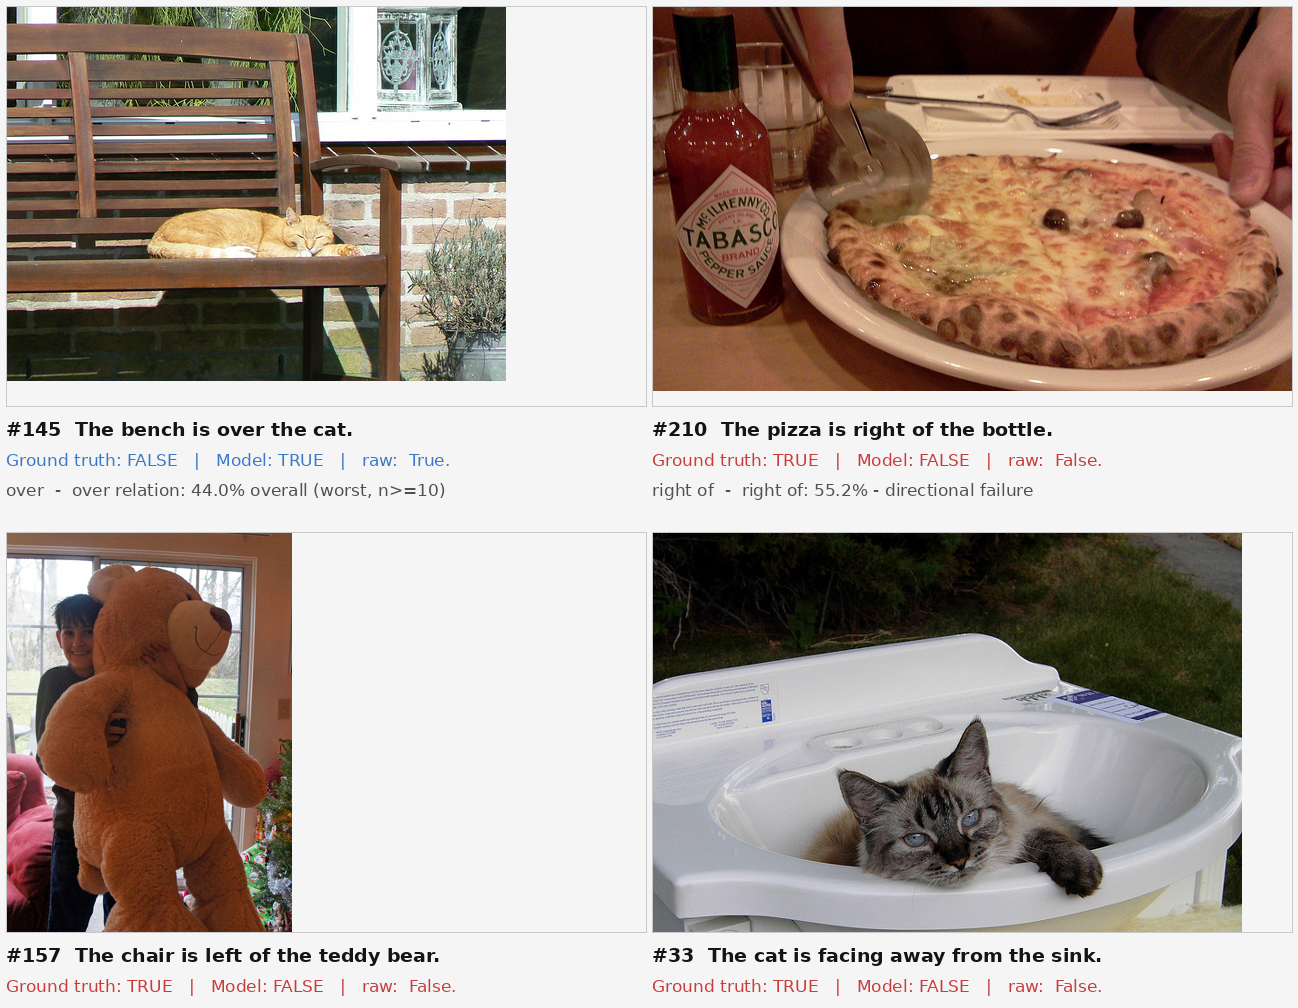
\includegraphics[width=\columnwidth]{fig/representative_failures.png}
\caption{Representative persistent failures (annotated grid; 15 cases).
Images: VSR test set. The dominant class is \emph{clear-image reasoning
failure}: the pose is obvious to a human and the model still errs.}
\label{fig:failures}
\end{figure}

\textbf{Transition counts.} Scaling (2B$\rightarrow$7B zero-shot): 28 both
wrong, 23 2B-wrong/7B-right, 22 2B-right/7B-wrong, 64 both right. Adaptation
(7B zero$\rightarrow$7B LoRA): 20 both wrong, 30 fixed, 27 broken, 60 both
right. Of the 48 annotated cases, hard-negative training fixes 5; 15 still
fail under all three 7B conditions. Facing/facing-away account for 68.8\% of
persistent failures.

% ============================================================
% G. Reproducibility and artifact index
% ============================================================
\section{Reproducibility and Artifact Index}
\label{app:repro}

Repo: \texttt{VLM-Spatial-Reasoning} (git). Every headline number in this
paper maps to a committed artifact; the audit script
\texttt{scripts/make\_paper\_figures.py} recomputes the main tables directly
from the raw prediction CSVs (output archived at
\texttt{paper/fig/audit\_output.txt}).

\begin{table*}[h]
\centering
\footnotesize
\setlength{\tabcolsep}{6pt}
\begin{tabular}{lll}
\toprule
Headline number & Artifact & Commit \\
\midrule
74.0 / 76.6 / 76.5 / 68.3 (2B) & \texttt{smolvlm2\_*\_metrics\_*.json} &
\texttt{35c1d16}, \texttt{1be61f3} \\
80.9 / 84.7 / 84.3 / 82.9 / 83.1 (7B) & \texttt{*\_metrics\_*.json} &
\texttt{37494b7}, \texttt{9fc694f}, \texttt{f1bc14f} \\
62.8 / 63.5 / 65.7 / 66.4 (orient.\ family) & same + prediction CSVs &
same \\
Per-relation cells (Table~1 (main)) & \texttt{orientation\_analysis.json} &
\texttt{2d732cd} \\
48-failure taxonomy & \texttt{orientation\_persistent\_*.json} &
\texttt{4b83729}, \texttt{1314e95} \\
Probe tables (App.~\ref{app:probes}) & \texttt{probe/*.json} &
\texttt{9d9c50c}, \texttt{fa9d0be}, \texttt{a0d50ca} \\
Two-stage (Table~3 (main)) & \texttt{two\_stage\_results.json} &
\texttt{1e83604} \\
Consistency (Fig.~2 (main)) & \texttt{consistency\_stats\_all.json} &
\texttt{6bf8b84} \\
Vision-side p-values & \texttt{vision\_side\_comparison.json} &
\texttt{f1bc14f} \\
SITE numbers & \texttt{site/zeroshot\_7b\_predictions.csv} & \texttt{8d7f173},
\texttt{b8336bb}, \texttt{46e3b49} \\
 & \texttt{site/zeroshot\_image\_metrics.json} & \\
\bottomrule
\end{tabular}
\caption{Headline-number $\rightarrow$ artifact $\rightarrow$ commit index (all
paths relative to \texttt{results/}).}
\label{tab:artifacts}
\end{table*}

\textbf{Environments.} VSR/7B and SITE runs: Ubuntu 24.04, Python 3.12.13,
torch 2.12.1+cu130, transformers 5.14.1, datasets 5.0.1, peft 0.20.0, 1$\times$
RTX A6000 (48\,GB). 2B runs: earlier python3.10-era environment (SmolVLM2
wrapper). No lock files exist; the adapter configs (committed) pin the LoRA
hyperparameters. Seeds: 42 defaults in 2B paths; single default seed elsewhere
--- per-run seeds are not recorded in the metrics JSONs (a known limitation).

\textbf{Canonical freeze.} The experimental result set is frozen at tag
\texttt{paper-freeze-v1}. Canonical tables are generated by
\texttt{scripts/build\_canonical\_tables.py}; clean-label results by
\texttt{scripts/clean\_label\_orientation.py}; publication figures by
\texttt{scripts/make\_publication\_figures.py}; SITE paired transfer statistics
by \texttt{scripts/compare\_site\_zeroshot\_lora.py}; VSR/SITE headline
recomputation by \texttt{scripts/make\_paper\_figures.py} (output archived at
\texttt{paper/fig/audit\_output.txt}).

\textbf{SITE artifact discrepancy.} The run-time metrics JSON
(\texttt{zeroshot\_image\_metrics.\allowbreak{}json}, commit \texttt{46e3b49})
and the canonical site table (\texttt{results/tables/site\_validation\_table.md})
report the secondary subset as $n{=}1{,}824$, raw 47.3\%, CAA 22.6\%; the
committed prediction CSV, consistent with the frozen protocol's image IDs,
yields $n{=}2{,}024$, raw 48.3\%, CAA 24.0\%. All other metrics (all/primary/
modality/source breakdowns) are bit-identical between the two artifacts. The
main paper reports the canonical-table values (47.3/22.6) and documents this
recomputation in a footnote; both values support the same conclusion.

\textbf{Data licenses/access.} VSR: \texttt{cambridgeltl/vsr\_random} (HF).
SITE: \texttt{franky-veteran/SITE-Bench}, CC-BY-4.0 (media in ~130\,GB zips;
requires HF read token). LoRA adapters are committed and loadable with peft;
base-model weights via HF Hub.

\textbf{Exact artifacts for the probe tables} (App.~\ref{app:probes}):
\texttt{results/probe/probe\_results.json},
\texttt{results/probe/patch\_probe\_results.json},
\texttt{results/probe/grounded\_probe\_results.json},
\texttt{results/probe/clear\_subset\_results.json},
\texttt{results/probe/grounded\_boxes.json}.
